\documentclass{article}\usepackage[]{graphicx}\usepackage[]{color}
%% maxwidth is the original width if it is less than linewidth
%% otherwise use linewidth (to make sure the graphics do not exceed the margin)
\makeatletter
\def\maxwidth{ %
  \ifdim\Gin@nat@width>\linewidth
    \linewidth
  \else
    \Gin@nat@width
  \fi
}
\makeatother

\definecolor{fgcolor}{rgb}{0.345, 0.345, 0.345}
\newcommand{\hlnum}[1]{\textcolor[rgb]{0.686,0.059,0.569}{#1}}%
\newcommand{\hlstr}[1]{\textcolor[rgb]{0.192,0.494,0.8}{#1}}%
\newcommand{\hlcom}[1]{\textcolor[rgb]{0.678,0.584,0.686}{\textit{#1}}}%
\newcommand{\hlopt}[1]{\textcolor[rgb]{0,0,0}{#1}}%
\newcommand{\hlstd}[1]{\textcolor[rgb]{0.345,0.345,0.345}{#1}}%
\newcommand{\hlkwa}[1]{\textcolor[rgb]{0.161,0.373,0.58}{\textbf{#1}}}%
\newcommand{\hlkwb}[1]{\textcolor[rgb]{0.69,0.353,0.396}{#1}}%
\newcommand{\hlkwc}[1]{\textcolor[rgb]{0.333,0.667,0.333}{#1}}%
\newcommand{\hlkwd}[1]{\textcolor[rgb]{0.737,0.353,0.396}{\textbf{#1}}}%
\let\hlipl\hlkwb

\usepackage{framed}
\makeatletter
\newenvironment{kframe}{%
 \def\at@end@of@kframe{}%
 \ifinner\ifhmode%
  \def\at@end@of@kframe{\end{minipage}}%
  \begin{minipage}{\columnwidth}%
 \fi\fi%
 \def\FrameCommand##1{\hskip\@totalleftmargin \hskip-\fboxsep
 \colorbox{shadecolor}{##1}\hskip-\fboxsep
     % There is no \\@totalrightmargin, so:
     \hskip-\linewidth \hskip-\@totalleftmargin \hskip\columnwidth}%
 \MakeFramed {\advance\hsize-\width
   \@totalleftmargin\z@ \linewidth\hsize
   \@setminipage}}%
 {\par\unskip\endMakeFramed%
 \at@end@of@kframe}
\makeatother

\definecolor{shadecolor}{rgb}{.97, .97, .97}
\definecolor{messagecolor}{rgb}{0, 0, 0}
\definecolor{warningcolor}{rgb}{1, 0, 1}
\definecolor{errorcolor}{rgb}{1, 0, 0}
\newenvironment{knitrout}{}{} % an empty environment to be redefined in TeX

\usepackage{alltt}
\usepackage{graphicx}
\usepackage[margin=1in]{geometry}
\usepackage{lscape}
\IfFileExists{upquote.sty}{\usepackage{upquote}}{}
\begin{document}



\section*{Problem 1}

\begin{knitrout}
\definecolor{shadecolor}{rgb}{0.969, 0.969, 0.969}\color{fgcolor}\begin{kframe}
\begin{alltt}
\hlkwd{set.seed}\hlstd{(}\hlnum{08544}\hlstd{)}
\hlcom{# N <- c(10000, 100000, 250000, 300000, 450000, 600000, 1000000, 1500000, 2000000, 2500000)}
\hlstd{N} \hlkwb{<-} \hlkwd{c}\hlstd{(}\hlnum{10000}\hlstd{,} \hlnum{100000}\hlstd{,} \hlnum{250000}\hlstd{,} \hlnum{300000}\hlstd{,} \hlnum{450000}\hlstd{,} \hlnum{600000}\hlstd{)}

\hlstd{ps} \hlkwb{<-} \hlkwd{c}\hlstd{()}
\hlstd{x} \hlkwb{<-} \hlkwd{c}\hlstd{()}
\hlstd{meanx} \hlkwb{<-} \hlkwd{c}\hlstd{()}
\hlstd{meany} \hlkwb{<-} \hlkwd{c}\hlstd{()}
\hlstd{y} \hlkwb{<-} \hlkwd{c}\hlstd{()}
\hlkwa{for} \hlstd{(i} \hlkwa{in} \hlnum{1}\hlopt{:}\hlkwd{length}\hlstd{(N))\{}
  \hlstd{e} \hlkwb{<-} \hlkwd{rnorm}\hlstd{(N[i],} \hlnum{0}\hlstd{,} \hlkwc{sd} \hlstd{=} \hlnum{0.01}\hlstd{)}
  \hlstd{x} \hlkwb{<-} \hlkwd{rnorm}\hlstd{(N[i],} \hlnum{0}\hlstd{,} \hlkwc{sd} \hlstd{=} \hlnum{0.01}\hlstd{)}
  \hlstd{y} \hlkwb{<-} \hlnum{3} \hlopt{+} \hlnum{0.01}\hlopt{*}\hlstd{x} \hlopt{+} \hlstd{e}
  \hlstd{meanx} \hlkwb{<-} \hlkwd{c}\hlstd{(meanx,} \hlkwd{mean}\hlstd{(x))}
  \hlstd{meany} \hlkwb{<-} \hlkwd{c}\hlstd{(meany,} \hlkwd{mean}\hlstd{(y))}
  \hlkwd{summary}\hlstd{(}\hlkwd{lm}\hlstd{(y} \hlopt{~} \hlstd{x))}
  \hlstd{ps[i]} \hlkwb{<-} \hlkwd{summary}\hlstd{(}\hlkwd{lm}\hlstd{(y} \hlopt{~} \hlstd{x))}\hlopt{$}\hlstd{coefficients[}\hlnum{2}\hlstd{,}\hlnum{4}\hlstd{]}
\hlstd{\}}

\hlkwd{cor}\hlstd{(x,y)}
\hlkwd{plot}\hlstd{(x[}\hlnum{1}\hlopt{:}\hlnum{100}\hlstd{], y[}\hlnum{1}\hlopt{:}\hlnum{100}\hlstd{],}
     \hlkwc{main} \hlstd{=} \hlstr{"Weak relationship between x and y"}\hlstd{,}
     \hlkwc{xlab} \hlstd{=} \hlstr{"100 x"}\hlstd{,}
     \hlkwc{ylab} \hlstd{=} \hlstr{'100 y'}\hlstd{)}
\end{alltt}
\end{kframe}
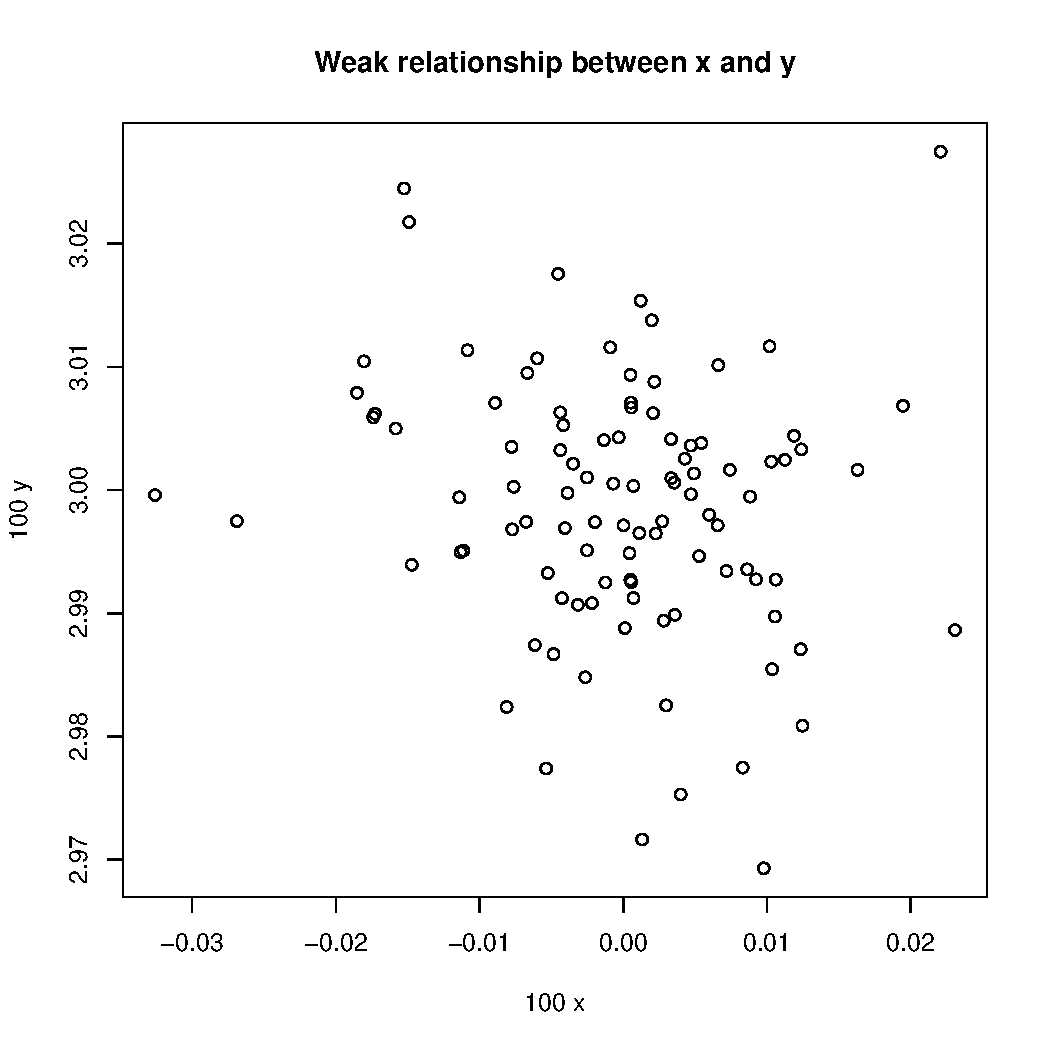
\includegraphics[width=4in]{figure/p1-1} 
\begin{kframe}\begin{alltt}
\hlcom{#hist(y)}
\hlkwd{plot}\hlstd{(N, ps,}
     \hlkwc{main} \hlstd{=} \hlstr{"P-values vs Number of observations"}\hlstd{,}
     \hlkwc{ylab} \hlstd{=} \hlstr{"p-values"}\hlstd{,}
     \hlkwc{xlab} \hlstd{=} \hlstr{"num observations"}
\hlstd{)}
\hlkwd{abline}\hlstd{(}\hlkwc{h} \hlstd{=} \hlnum{.05}\hlstd{)}
\end{alltt}
\end{kframe}
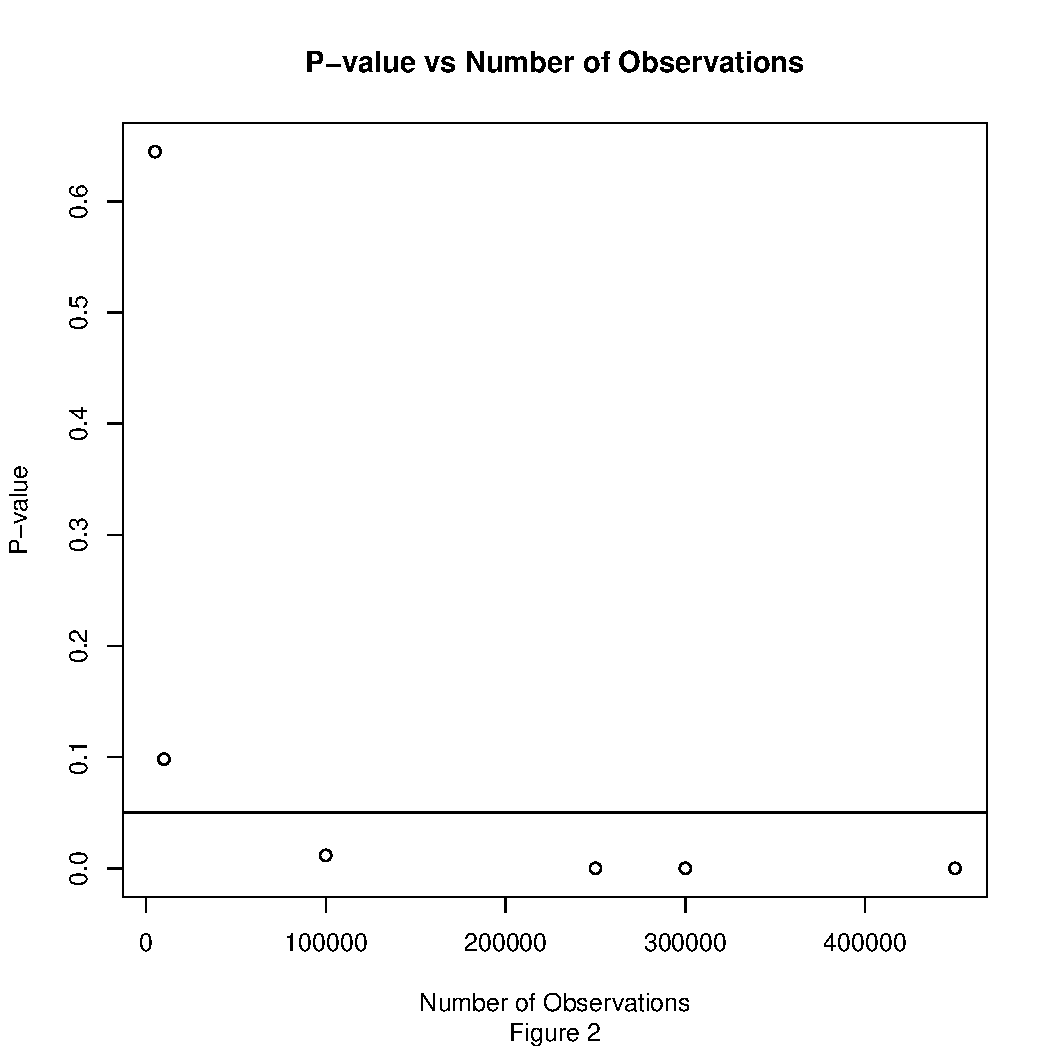
\includegraphics[width=4in]{figure/p1-2} 
\begin{kframe}\begin{alltt}
\hlcom{#cor(x, y)}
\hlcom{#N[ps < 0.05]}
\end{alltt}
\end{kframe}
\end{knitrout}

\noindent We set the parameters to $y = 3 + 0.01*x + e$, for which y has a weak relationship with x.  The correlation is 0.009. We then ran regressions on samples of increasing size, from 10000 to NA and plotted the p-values for each regression.  As seen in the figure, the relationship is consistently statistically significant after 1000000 samples, which shows that as sample size increases, even weak relationships will be shown as significant.


\section*{Problem 2}

\begin{knitrout}
\definecolor{shadecolor}{rgb}{0.969, 0.969, 0.969}\color{fgcolor}\begin{kframe}
\begin{alltt}
\hlkwd{set.seed}\hlstd{(}\hlnum{08544}\hlstd{)}
\hlstd{N.p2} \hlkwb{<-} \hlnum{1000}
\hlcom{#x1 is asian}
\hlstd{x1} \hlkwb{<-} \hlkwd{rbinom}\hlstd{(N.p2,} \hlkwc{size} \hlstd{=} \hlnum{1}\hlstd{,} \hlkwc{prob} \hlstd{=} \hlnum{.056}\hlstd{)}
\hlcom{#hist(x1)}
\hlcom{#personality "personality"}
\hlstd{x2} \hlkwb{<-} \hlkwd{rnorm}\hlstd{(N.p2, (}\hlnum{5} \hlopt{-} \hlstd{x1}\hlopt{*}\hlnum{3}\hlstd{),} \hlnum{1.5}\hlstd{)}
\hlcom{#hist(x2)}
\hlcom{#not get into harvard?}
\hlstd{y} \hlkwb{<-} \hlkwd{plogis}\hlstd{(x2} \hlopt{-} \hlnum{6}\hlstd{)}
\hlcom{#hist(y)}

\hlkwd{summary}\hlstd{(}\hlkwd{lm}\hlstd{(y} \hlopt{~} \hlstd{x2} \hlopt{+} \hlstd{x1))}
\hlkwd{cor}\hlstd{(x1, y)}
\end{alltt}
\end{kframe}
\end{knitrout}
\noindent We completed Problem 2b prior to 2a, which is why the code is nearly identical. The correlation between x1 and y is -0.252, while the coefficient in the regression is 0.191, showing that the lurking variable x2 changes the sign.\\

\begin{knitrout}
\definecolor{shadecolor}{rgb}{0.969, 0.969, 0.969}\color{fgcolor}\begin{kframe}
\begin{alltt}
\hlkwd{set.seed}\hlstd{(}\hlnum{08544}\hlstd{)}
\hlstd{N.p2} \hlkwb{<-} \hlnum{1000}
\hlcom{#asian is asian}
\hlstd{asian} \hlkwb{<-} \hlkwd{rbinom}\hlstd{(N.p2,} \hlkwc{size} \hlstd{=} \hlnum{1}\hlstd{,} \hlkwc{prob} \hlstd{=} \hlnum{.056}\hlstd{)}
\hlcom{#hist(asian)}
\hlcom{#personality "personality"}
\hlstd{personality} \hlkwb{<-} \hlkwd{rnorm}\hlstd{(N.p2, (}\hlnum{5} \hlopt{-} \hlstd{asian}\hlopt{*}\hlnum{3}\hlstd{),} \hlnum{1.5}\hlstd{)}
\hlcom{#hist(personality)}
\hlcom{#not get into harvard?}
\hlstd{harvard} \hlkwb{<-} \hlkwd{plogis}\hlstd{(personality} \hlopt{-} \hlnum{6}\hlstd{)}
\hlcom{#hist(harvard)}

\hlkwd{summary}\hlstd{(}\hlkwd{lm}\hlstd{(harvard} \hlopt{~} \hlstd{personality} \hlopt{+} \hlstd{asian))}
\hlkwd{cor}\hlstd{(asian, harvard)}
\end{alltt}
\end{kframe}
\end{knitrout}

\noindent We chose to comment on the Harvard Circut Court decision on admission of Asian American applicants.  Here, x1 is binomially distributed to mark if the candidate is Asian (5.6\% of the U.S. population is Asian).  x2 is the ``personality'' score as described in the brief, which here is lowered if the applicant is Asian. y is the probability of acceptance to Harvard based on the personality score distribution, which is lower for Asian applicants. \pagebreak

\section*{Problem 3}
\subsection*{Part a}
\begin{figure}[h!]
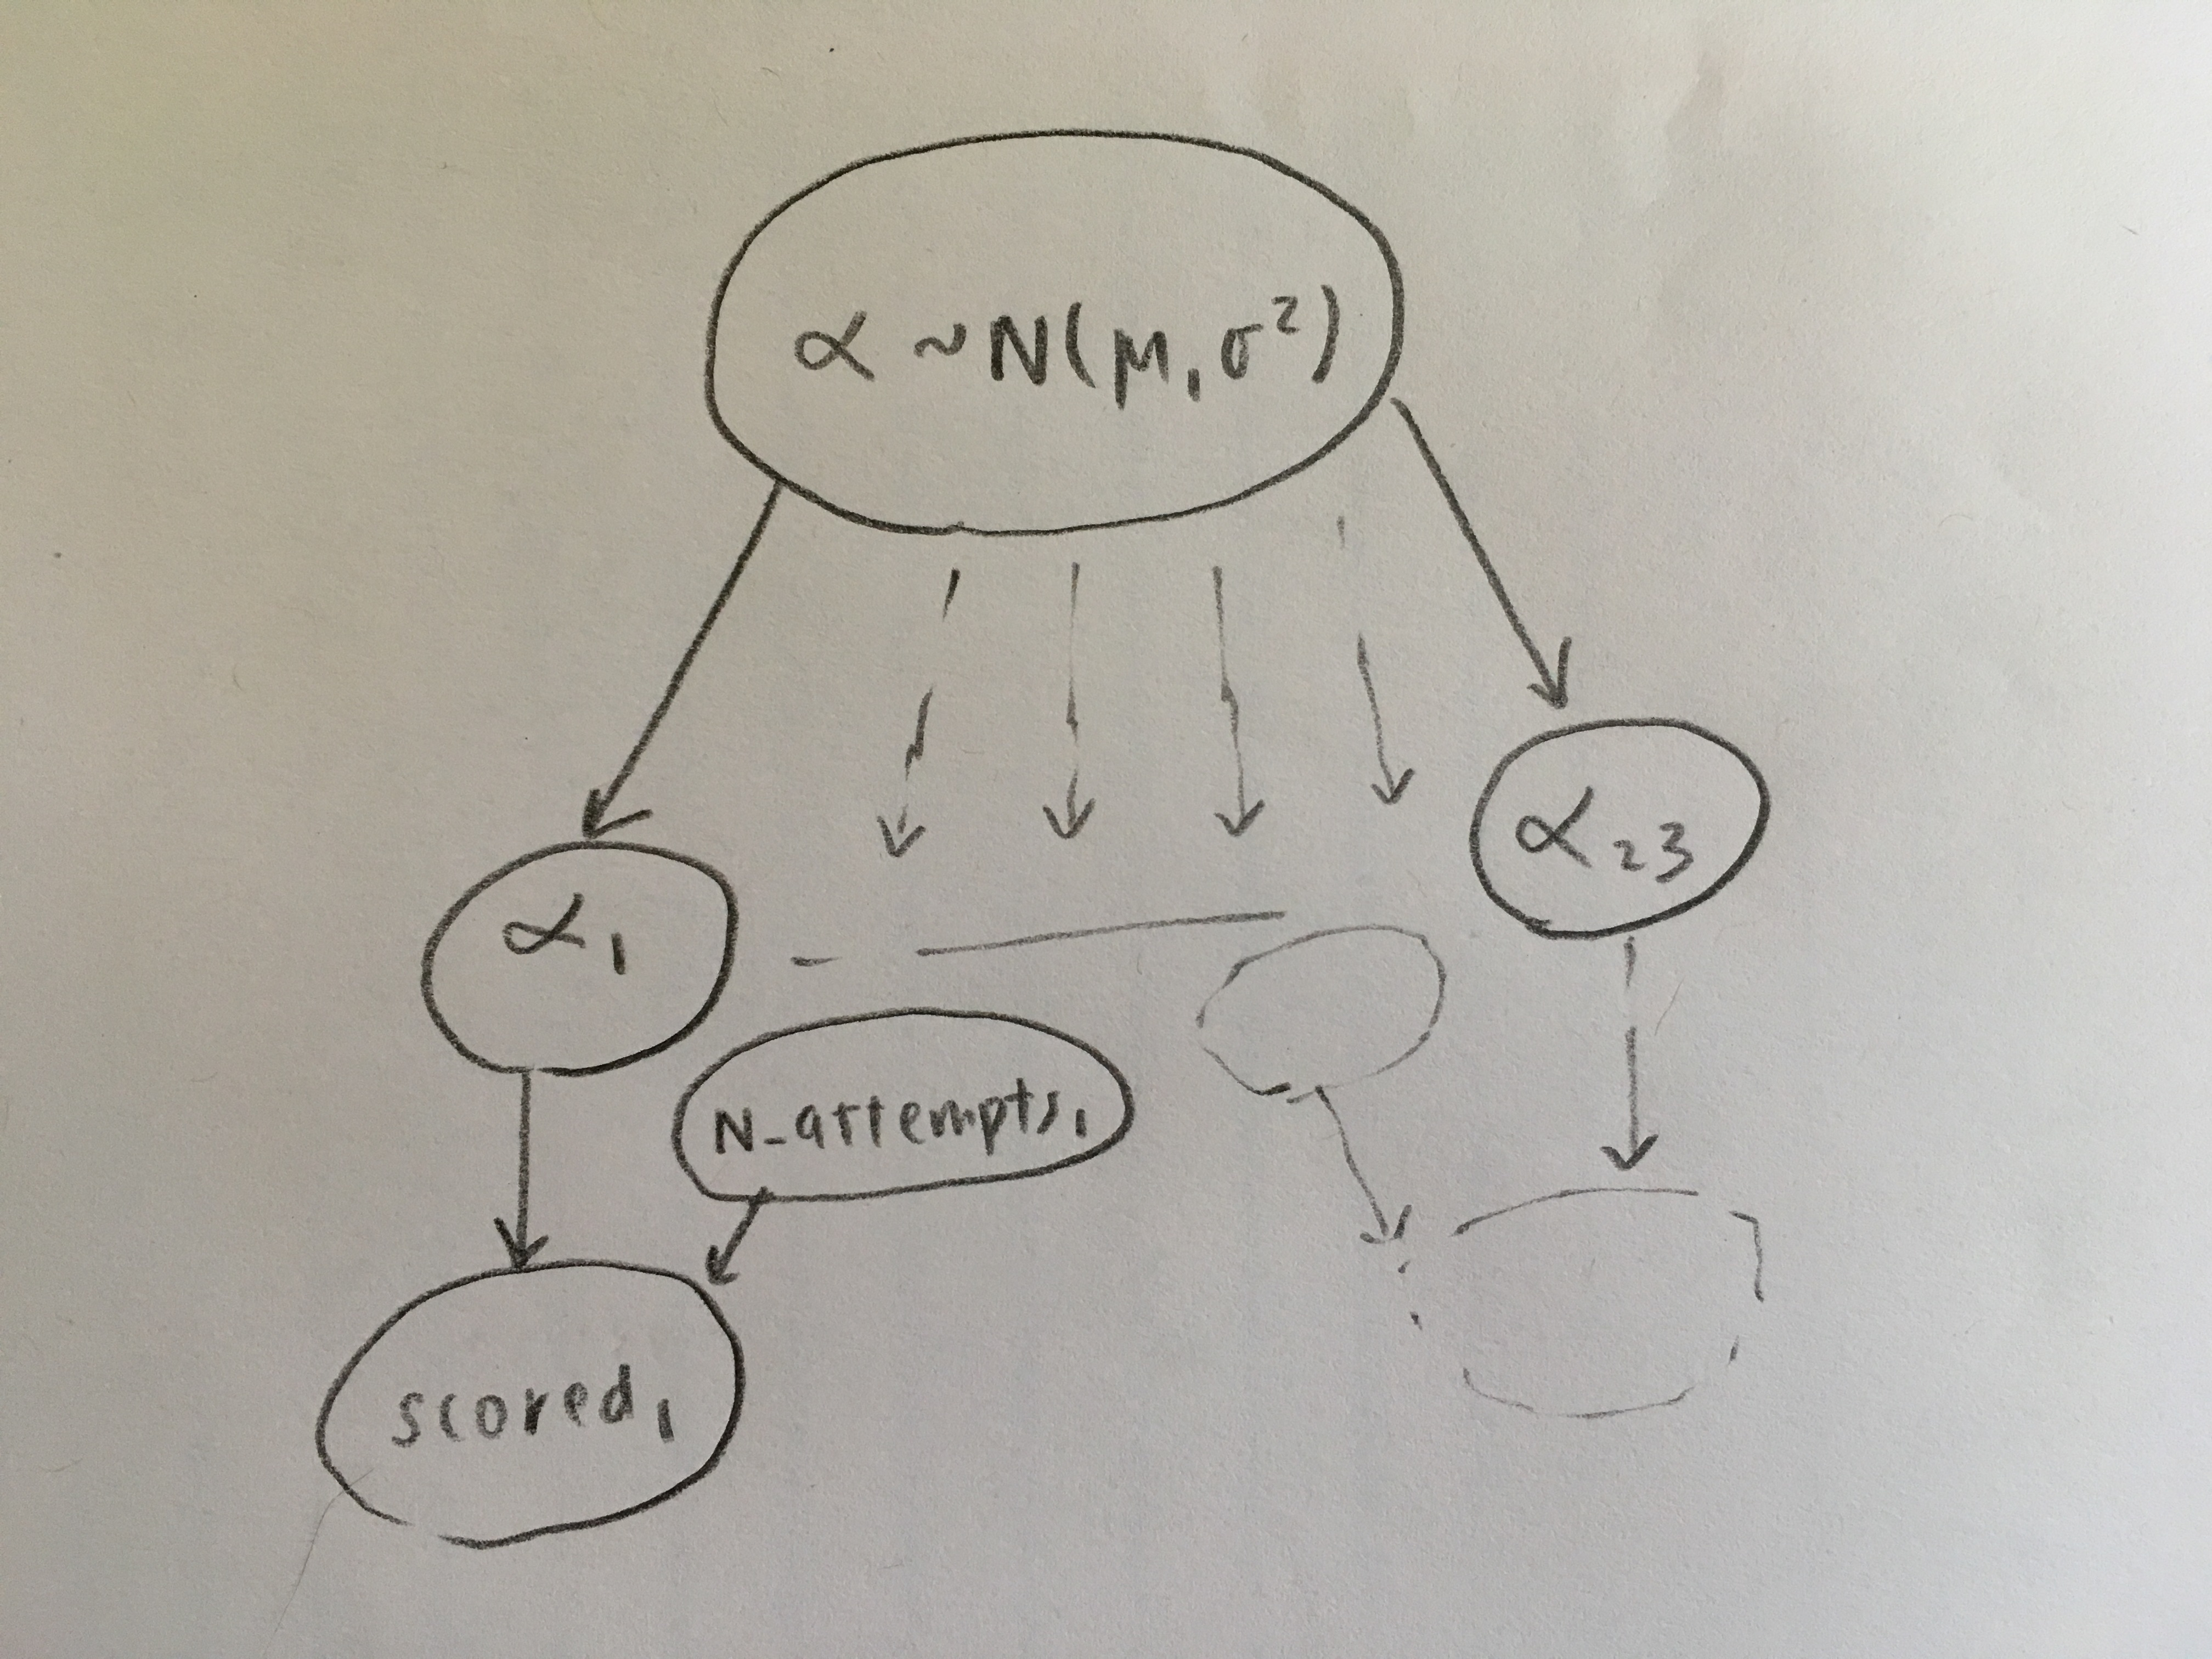
\includegraphics[scale=.1]{/Users/mikakoinaba/Desktop/sml310_mp1/p3a.jpg}
\end{figure}

\subsection*{Part b}

% N = game number
% scored[N] = array of scores indexed by game
% attempted[N] = array of number of attemps indexed by game

% mu = overall average skill level
% sigma = overall stdev of skill level, lower bounded by 0

% alpha[N] = array of average skill level indexed by game
% loop samples from ~N(mu, sigma^2)

% alpha_norm ~ N(0, 1)
% scored sum of bernoulli of attempted using prob of alpha(skill level)

\begin{knitrout}
\definecolor{shadecolor}{rgb}{0.969, 0.969, 0.969}\color{fgcolor}\begin{kframe}
\begin{alltt}
\hlstd{lines} \hlkwb{<-}
\hlstr{"Game   Scored  N.Attempts
1   4   5
2   5   11
3   5   14
4   5   12
5   2   7
6   7   10
7   6   14
8   9   15
9   4   12
10  1   4
11  13  27
12  5   17
13  6   12
14  9   9
15  7   12
16  3   10
17  8   12
18  1   6
19  18  39
20  3   13
21  10  17
22  1   6
23  3   12"}
\hlstd{con} \hlkwb{<-} \hlkwd{textConnection}\hlstd{(lines)}
\hlstd{shaq} \hlkwb{<-} \hlkwd{read.csv}\hlstd{(con,} \hlkwc{sep}\hlstd{=}\hlstr{""}\hlstd{)}
\hlstd{shaq}

\hlcom{# partial pooling: each alpha affected by overall alpha}
\hlstd{shaq_model_stan} \hlkwb{<-} \hlstr{"
data\{
  // data we supply
  int<lower=0> N; // game number, must be positive
  int scored[N]; // array of scores indexed by game
  int attempted[N]; // array of number of attempts indexed by games
\}

parameters\{
  real mu; // overall average skill level
  real<lower=0> sigma; // overall stdev of skill level, lower bounded by 0
  vector[N] alpha_norm; // array of 'zscores'
\}

transformed parameters\{
  real alpha[N]; // array of average skill level indexed by game
                 // produced using alpha_norms
  for(n in 1:N)
    alpha[n] = mu + sigma * alpha_norm[n];
\}

model\{
  alpha_norm ~ normal(0, 1);
  scored ~ binomial(attempted, inv_logit(alpha)); // scored modeled using num attempted & 0 - 1 of alpha
\}"}

\hlstd{adaptSteps} \hlkwb{=} \hlnum{1000}            \hlcom{# Number of steps to "tune" the samplers.}
\hlstd{burnInSteps} \hlkwb{=} \hlnum{5000}           \hlcom{# Number of steps to "burn-in" the samplers.}
\hlstd{nChains} \hlkwb{=} \hlnum{3}                  \hlcom{# Number of chains to run.}
\hlstd{numSavedSteps}\hlkwb{=}\hlnum{12000}          \hlcom{# Total number of steps in chains to save.}
\hlstd{thinSteps}\hlkwb{=}\hlnum{10}                 \hlcom{# Number of steps to "thin" (1=keep every step).}

\hlstd{shaq_model} \hlkwb{<-} \hlkwd{stan_model}\hlstd{(}\hlkwc{model_code} \hlstd{= shaq_model_stan,} \hlkwc{model_name} \hlstd{=} \hlstr{"shaq_model"}\hlstd{)}
\hlstd{shaq_fit} \hlkwb{<-} \hlkwd{sampling}\hlstd{(}\hlkwc{object}\hlstd{=shaq_model,}
                      \hlkwc{data} \hlstd{=} \hlkwd{list}\hlstd{(}\hlkwc{N}\hlstd{=}\hlkwd{nrow}\hlstd{(shaq),} \hlkwc{scored}\hlstd{=shaq}\hlopt{$}\hlstd{Scored,} \hlkwc{attempted} \hlstd{= shaq}\hlopt{$}\hlstd{N.Attempts),}
                      \hlkwc{chains} \hlstd{= nChains,}
                      \hlkwc{iter} \hlstd{= (}\hlkwd{ceiling}\hlstd{(numSavedSteps}\hlopt{/}\hlstd{nChains)}\hlopt{*}\hlstd{thinSteps}
                               \hlopt{+} \hlstd{burnInSteps),}
                      \hlkwc{warmup} \hlstd{= burnInSteps,}
                      \hlkwc{thin} \hlstd{= thinSteps,}
                      \hlkwc{init} \hlstd{=} \hlstr{"random"}\hlstd{)}

\hlstd{samplesPartial} \hlkwb{<-} \hlkwd{extract}\hlstd{(shaq_fit)}

\hlcom{# posterior distribution for each parameter}
\hlcom{# hist(samplesPartial$mu) # prob distribution of mu}
\hlcom{# hist(samplesPartial$sigma) # prob distribution of sigma}
\hlcom{# hist(samplesPartial$alpha[, 1]) # prob distribution of alpha_1}
\hlcom{# hist(samplesPartial$alpha[, 2]) # prob distribution of alpha_2}
\hlcom{# 95% of data lies within 2 stdev of the mean 0 --> }
\hlstd{good} \hlkwb{<-} \hlkwd{plogis}\hlstd{(}\hlkwd{mean}\hlstd{(samplesPartial}\hlopt{$}\hlstd{mu)} \hlopt{+} \hlnum{2} \hlopt{*} \hlkwd{mean}\hlstd{(samplesPartial}\hlopt{$}\hlstd{sigma))}
\hlstd{bad} \hlkwb{<-} \hlkwd{plogis}\hlstd{(}\hlkwd{mean}\hlstd{(samplesPartial}\hlopt{$}\hlstd{mu)} \hlopt{-} \hlnum{2} \hlopt{*} \hlkwd{mean}\hlstd{(samplesPartial}\hlopt{$}\hlstd{sigma))}
\hlstd{good}
\hlstd{bad}

\hlstd{N} \hlkwb{<-} \hlnum{23}
\hlstd{conf_data} \hlkwb{<-} \hlkwd{data.frame}\hlstd{(}\hlkwc{games} \hlstd{=} \hlnum{1}\hlopt{:}\hlstd{N,} \hlkwc{mean} \hlstd{=} \hlnum{NA}\hlstd{,} \hlkwc{upper} \hlstd{=} \hlnum{NA}\hlstd{,} \hlkwc{lower} \hlstd{=} \hlnum{NA}\hlstd{)}

\hlkwa{for} \hlstd{(i} \hlkwa{in} \hlnum{1}\hlopt{:}\hlstd{N)\{}
  \hlstd{conf_data[i,} \hlstr{"mean"}\hlstd{]} \hlkwb{=} \hlkwd{mean}\hlstd{(samplesPartial}\hlopt{$}\hlstd{alpha[, i])}
  \hlstd{conf_data[i,} \hlstr{"upper"}\hlstd{]} \hlkwb{=} \hlkwd{mean}\hlstd{(samplesPartial}\hlopt{$}\hlstd{alpha[, i])} \hlopt{+} \hlnum{2} \hlopt{*} \hlkwd{sd}\hlstd{(samplesPartial}\hlopt{$}\hlstd{alpha[, i])}
  \hlstd{conf_data[i,} \hlstr{"lower"}\hlstd{]} \hlkwb{=} \hlkwd{mean}\hlstd{(samplesPartial}\hlopt{$}\hlstd{alpha[, i])} \hlopt{-} \hlnum{2} \hlopt{*} \hlkwd{sd}\hlstd{(samplesPartial}\hlopt{$}\hlstd{alpha[, i])}
\hlstd{\}}


\hlkwd{ggplot}\hlstd{(conf_data)} \hlopt{+}
  \hlkwd{geom_segment}\hlstd{(}\hlkwd{aes}\hlstd{(}\hlkwc{x}\hlstd{=lower,}\hlkwc{y}\hlstd{=games,}\hlkwc{xend}\hlstd{=upper,}\hlkwc{yend}\hlstd{=games),}
               \hlkwc{arrow}\hlstd{=}\hlkwd{arrow}\hlstd{(}\hlkwc{length}\hlstd{=}\hlkwd{unit}\hlstd{(}\hlnum{0.1}\hlstd{,}\hlstr{"cm"}\hlstd{),}
                           \hlkwc{ends}\hlstd{=}\hlstr{'both'}\hlstd{),}\hlkwc{size}\hlstd{=}\hlnum{.1}\hlstd{)} \hlopt{+}
  \hlkwd{labs}\hlstd{(}\hlkwc{x} \hlstd{=} \hlstr{"Confidence Interval"}\hlstd{,} \hlkwc{y} \hlstd{=} \hlstr{"Game"}\hlstd{,}
       \hlkwc{title} \hlstd{=} \hlstr{"95% predictive interval - partial pooling"}\hlstd{)}
\end{alltt}
\end{kframe}
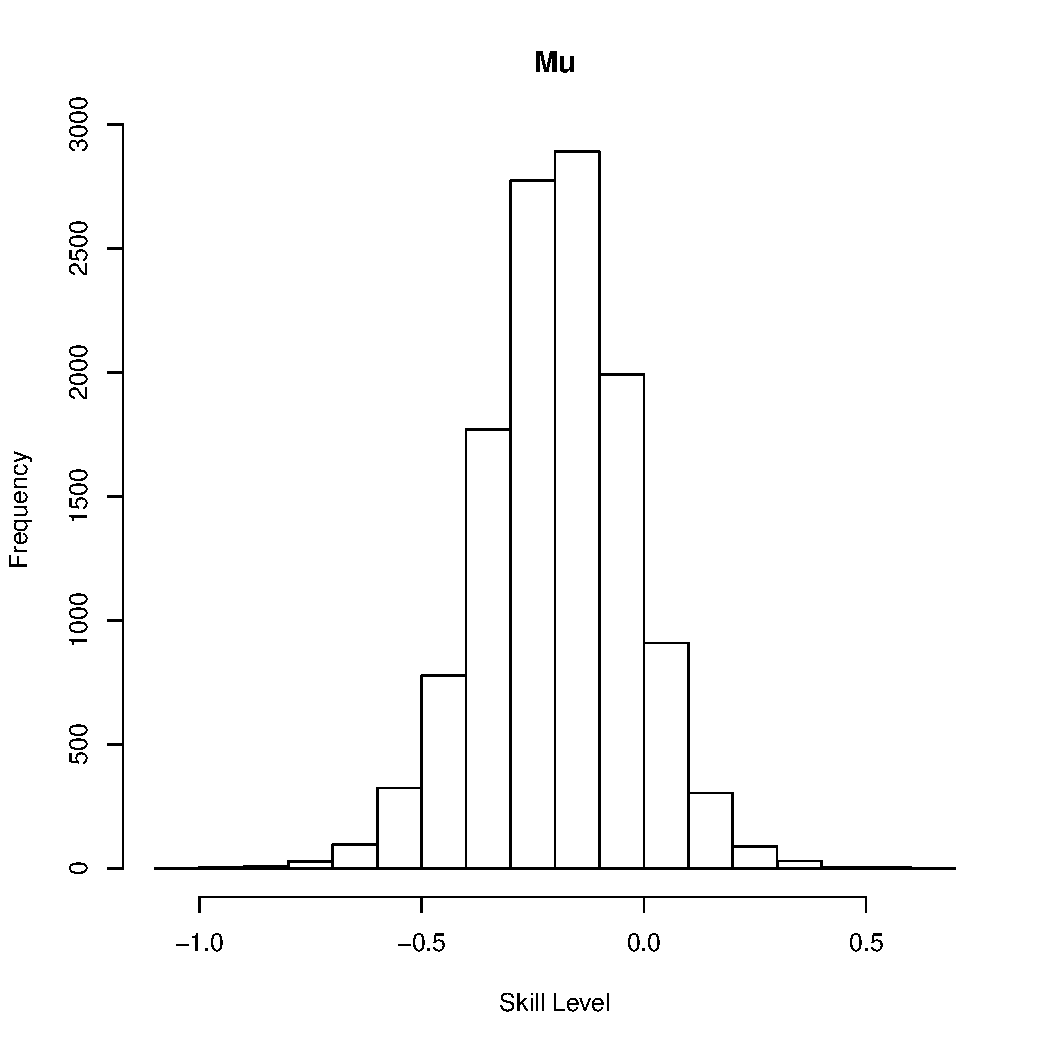
\includegraphics[width=4in]{figure/p3b-1} 
\begin{kframe}\begin{alltt}
\hlcom{#ggplot(conf_data, aes(x = games, y = mean)) +  }
 \hlcom{# geom_errorbar(aes(ymin=lower, ymax=upper))}
\end{alltt}
\end{kframe}
\end{knitrout}

\begin{knitrout}
\definecolor{shadecolor}{rgb}{0.969, 0.969, 0.969}\color{fgcolor}\begin{kframe}
\begin{alltt}
\hlkwd{par}\hlstd{(}\hlkwc{mfrow}\hlstd{=}\hlkwd{c}\hlstd{(}\hlnum{2}\hlstd{,} \hlnum{2}\hlstd{))}
\hlkwd{hist}\hlstd{(samplesPartial}\hlopt{$}\hlstd{mu,} \hlkwc{main} \hlstd{=} \hlstr{"mu"}\hlstd{)}
\hlkwd{hist}\hlstd{(samplesPartial}\hlopt{$}\hlstd{sigma,} \hlkwc{main} \hlstd{=} \hlstr{"sigma"}\hlstd{)}
\hlkwd{hist}\hlstd{(samplesPartial}\hlopt{$}\hlstd{alpha[,} \hlnum{1}\hlstd{],} \hlkwc{main} \hlstd{=}  \hlstr{"game 1"}\hlstd{)}
\hlkwd{hist}\hlstd{(samplesPartial}\hlopt{$}\hlstd{alpha[,} \hlnum{2}\hlstd{],} \hlkwc{main} \hlstd{=} \hlstr{"game 2"}\hlstd{)}
\end{alltt}
\end{kframe}
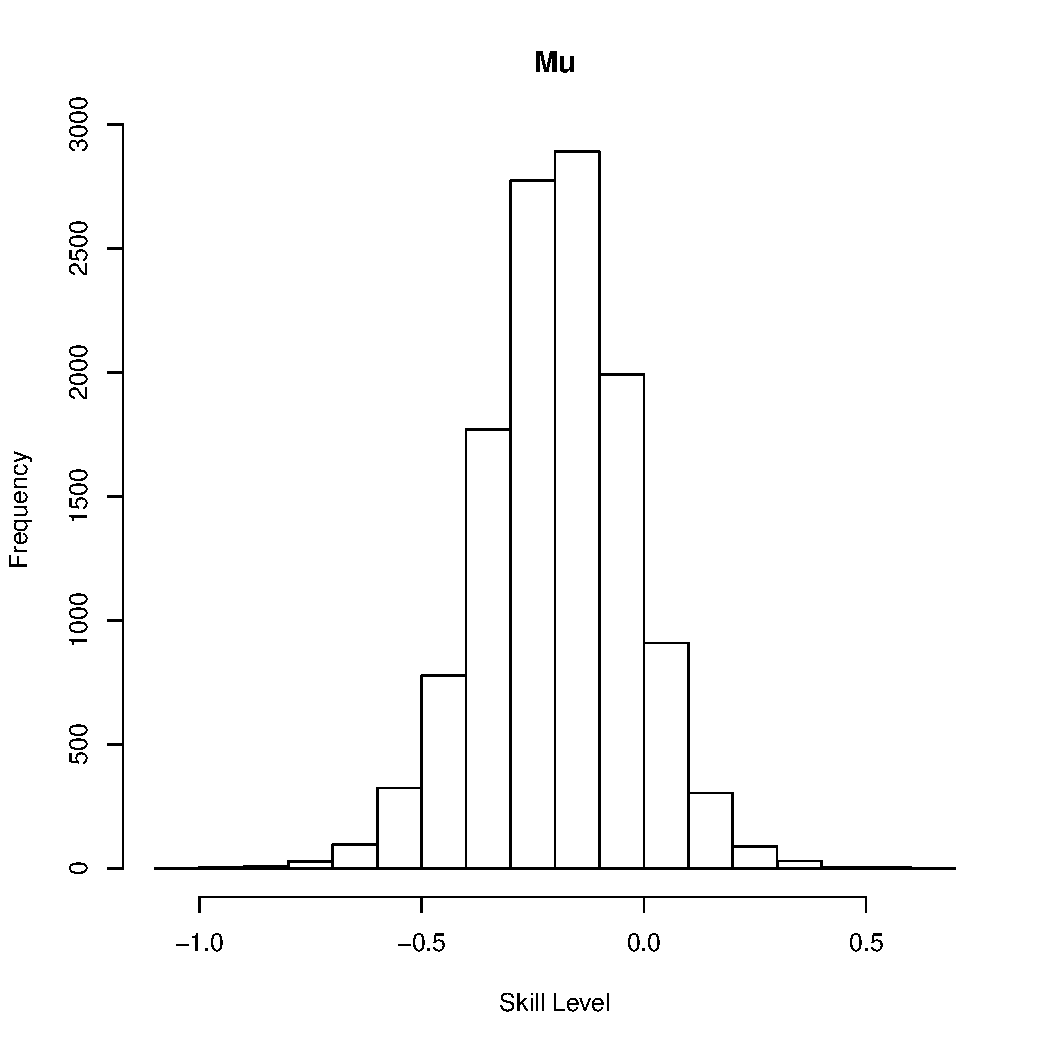
\includegraphics[width=4in]{figure/p3bHist-1} 

\end{knitrout}



\begin{knitrout}
\definecolor{shadecolor}{rgb}{0.969, 0.969, 0.969}\color{fgcolor}\begin{kframe}
\begin{alltt}
\hlcom{# plot an uniform dist of 0 for sigma}
\end{alltt}
\end{kframe}
\end{knitrout}



\begin{knitrout}
\definecolor{shadecolor}{rgb}{0.969, 0.969, 0.969}\color{fgcolor}\begin{kframe}
\begin{alltt}
\hlcom{# plot 20 for sigma}
\hlstd{sigma} \hlkwb{<-} \hlkwd{rep}\hlstd{(}\hlnum{0}\hlstd{,} \hlnum{12000}\hlstd{)} \hlcom{# it looked weird}

\hlkwd{par}\hlstd{(}\hlkwc{mfrow}\hlstd{=}\hlkwd{c}\hlstd{(}\hlnum{2}\hlstd{,} \hlnum{2}\hlstd{))}
\hlkwd{hist}\hlstd{(samplesNo}\hlopt{$}\hlstd{mu)}
\end{alltt}


{\ttfamily\noindent\bfseries\color{errorcolor}{\#\# Error in hist(samplesNo\$mu): object 'samplesNo' not found}}\begin{alltt}
\hlkwd{barplot}\hlstd{(}\hlkwd{length}\hlstd{(sigma), sigma,} \hlkwc{main} \hlstd{=} \hlstr{"sigma"}\hlstd{,} \hlkwc{names.arg} \hlstd{=} \hlstr{"20"}\hlstd{)}
\hlkwd{hist}\hlstd{(samplesNo}\hlopt{$}\hlstd{alpha[,} \hlnum{1}\hlstd{])}
\end{alltt}


{\ttfamily\noindent\bfseries\color{errorcolor}{\#\# Error in hist(samplesNo\$alpha[, 1]): object 'samplesNo' not found}}\begin{alltt}
\hlkwd{hist}\hlstd{(samplesNo}\hlopt{$}\hlstd{alpha[,} \hlnum{2}\hlstd{])} \hlcom{# they're all different}
\end{alltt}


{\ttfamily\noindent\bfseries\color{errorcolor}{\#\# Error in hist(samplesNo\$alpha[, 2]): object 'samplesNo' not found}}\end{kframe}
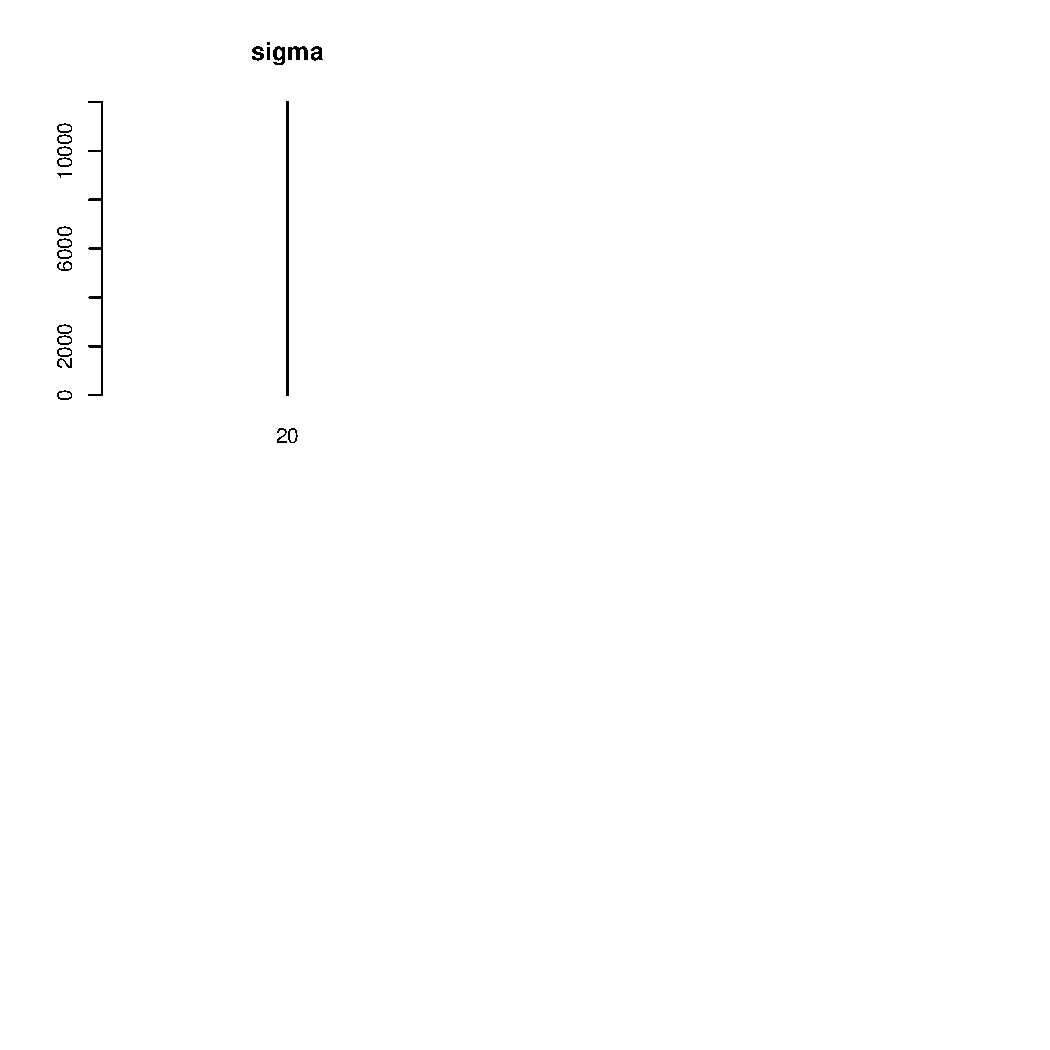
\includegraphics[width=4in]{figure/p3cNoHist-1} 

\end{knitrout}
\end{document}

